\newpage
\section{Concurrencia}


\subsection{Concurrencia de Cevianas}


\begin{figure}[htb]
    \centering
    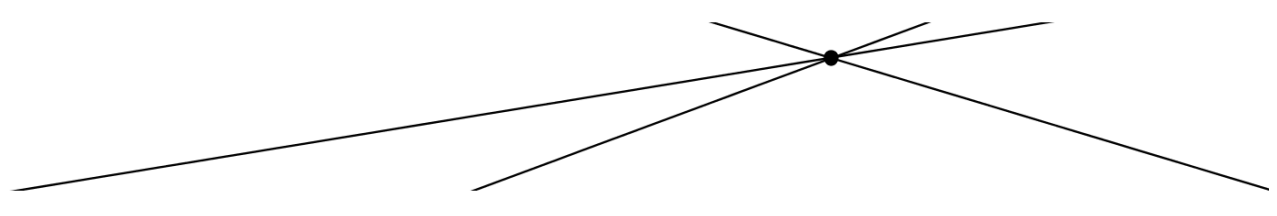
\includegraphics[width=14cm]{images/concurrence-1}
\end{figure}

Tres rectas son concurrentes si pasan por un punto común.
Sabiendo esto, veamos el primer hecho fundamental para abordar los problemas de concurrencia.

\begin{section-theorem.tcb}[\textbf{Teorema de Ceva}]
    Dado un triángulo $ABC$, sean $D$, $E$ y $F$ puntos sobre los lados $BC$, $CA$ y $AB$ (o sus prolongaciones), respectivamente.
    Entonces las rectas $AD$, $BE$ y $CF$ son concurrentes si y sólo si
    \begin{gather*}
        \frac{BD}{DC} \cdot \frac{CE}{EA} \cdot \frac{AF}{FB} = 1.
    \end{gather*}
\end{section-theorem.tcb}

A partir de este teorema se vuelve evidente la concurrencia de las principales rectas notables\footnote{Ver los ejercicios del 2.1 al 2.4.}.
De igual forma muchos otros problemas pueden ser resueltos por el teorema de Ceva, la dificultad radica en transformar las proporciones evidentes en otras que sean más fáciles de manipular para que el producto de todas sea igual a 1.

Es importante resaltar que la manipulación de razones con áreas no funciona, pues a partir de la manipulación de áreas también puede ser demostrado este teorema, y lo único que se obtendría es un avanze circular, por ello es mejor hacerlo con semejanza de triángulos, potencia de punto o trigonometría como se verá más adelante.

\begin{section-definition.tcb}
    A toda recta que parte del vértice hacia el lado opuesto se le denomina \textit{ceviana.}
\end{section-definition.tcb}

\begin{section-definition.tcb}[\textbf{Triángulo ceviano}]
    Para todo punto $P$, las cevianas desde $A$, $B$ y $C$ que pasan por $P$ y cortan a los lados opuestos en $A'$, $B'$ y $C'$.
    El triángulo $A'B'C'$ es el triángulo ceviano de $P$ y sus vértices se llaman trazas cevianas de $P$.
\end{section-definition.tcb}

\begin{section-theorem.tcb}[\textbf{Ceva trigonométrico}]
    Las rectas $AD$, $BE$ y $CF$ son cevianas concurrentes del triángulo $ABC$ si y sólo si
    \begin{gather*}
        \frac{sen(\angle BAD)}{sen(\angle DAC)} \cdot \frac{sen(\angle CBE)}{sen(\angle EBA)} \cdot \frac{sen(\angle ACF)}{sen(\angle FCB)} = 1.
    \end{gather*}
\end{section-theorem.tcb}

La manipulación trigonométrica del teorema de Ceva se vuelve muy importante a la hora de enfrentarse a problemas que pueden parecer práticamente inaccesibles, pues es más general y más aplicable que la semajanza de triángulos.

\begin{section-definition.tcb}[\textbf{El punto de Gergonne}]
    Sea $ABC$ un triángulo, y sean $D$, $E$ y $F$ los puntos de tangencia del incírculo con $BC$, $CA$ y $AB$, respectivamente.
    Entonces, $AD$, $BE$ y $CF$ son concurrentes.
\end{section-definition.tcb}

\begin{section-definition.tcb}[\textbf{El punto de Nagel}]
    Sea $ABC$ un triángulo, y sean $D'$, $E'$ y $F'$ los puntos de tangencia de los excírculos respectivos a $A$, $B$ y $C$ con $BC$, $CA$ y $AB$, respectivamente.
    Entonces, $AD'$, $BE'$ y $CF'$ son concurrentes.
\end{section-definition.tcb}


\begin{section-theorem.tcb}[\textbf{Teorema de Ceva sobre la circunferencia}]
    Sean $ABC$ y $DEF$ dos triángulos sobre la misma circunferencia.
    Entonces las rectas $AD$, $BE$ y $CF$ son concurrentes si y sólo si
    \[\frac{BD}{DC} \cdot \frac{CE}{EA} \cdot \frac{AF}{FB} = 1.\]
\end{section-theorem.tcb}

\begin{section-definition.tcb}[\textbf{Triángulo circunceviano}]
    A todo punto que no esté sobre alguno de los lados de un triángulo dado es posible asignarle un nuevo triángulo, que surge a partir de la intersección de las cevianas con el circuncírculo del triángulo.
\end{section-definition.tcb}

\begin{section-theorem.tcb}[\textbf{Teorema de Steinbart}]
    Sea $ABC$ un triángulo, $D$, $E$ y $F$ los puntos de tanagencia del incírculo con los lados $BC$, $CA$ y $AB$, respectivamente.
    Sean $P$, $Q$ y $R$ puntos sobre el incírculo de $ABC$.
    Llamemos $A'$, $B'$ y $C'$ las intersecciones de $EF$ con $PD$, $DF$ con $QE$ y $DE$ con $FR$.
    Entonces $AP$, $BQ$ y $CR$ son concurrentes si y sólo si $DP$, $EQ$ y $FR$ son concurrentes.
\end{section-theorem.tcb}

\begin{section-theorem.tcb}[\textbf{Teorema de Jacobi}]
    Sea $ABC$ un triángulo, y sean $X$, $Y$, $Z$ tres puntos en el plano tales que $\angle YAC = \angle BAZ$, $\angle ZBA = \angle CBX$, $\angle XCB = \angle ACY$.
    Entonces las rectas $AX$, $BY$ y $CZ$ son concurrentes.
\end{section-theorem.tcb}

\begin{section-definition.tcb}[\textbf{Puntos isotómicos}]
    Dos puntos son isotómicos si estos coinciden al ser reflejados por el punto medio del segmento al que pertenecen.
\end{section-definition.tcb}

\begin{section-definition.tcb}[\textbf{Conjugados isotómicos}]
    Dado un triángulo $ABC$ se tienen tres cevianas $AD$, $BE$ y $CF$ las cuales son concurrentes en un punto $P$.
    Sean $D'$, $E'$ y $F'$ las reflexiones de $D$, $E$ y $F$ sobre los puntos medios de $BC$, $CA$ y $AB$ respectivamente.
    Entonces las rectas $AD'$, $BE'$ y $CF'$ son concurrentes.
\end{section-definition.tcb}

\begin{section-definition.tcb}[\textbf{Cevianas isogonales}]
    Dos cevianas son isogonales del $\triangle ABC$ si ambas parte del mismo vértice del triángulo y una es la reflexión de la otra con respecto a la bisectriz interna de $\triangle ABC$.
\end{section-definition.tcb}

\begin{section-definition.tcb}[\textbf{Conjugados isogonales}]
    Dado un triángulo $ABC$ se tienen tres cevianas $AD$, $BE$ y $CF$ las cuales son concurrentes en un punto $P$.
    Sean $AD'$, $BE'$ y $CF'$ las reflexiones de $AD$, $BE$ y $CF$ sobre las bisectrices de $\angle A$, $\angle B$ y $\angle C$ respectivamente.
    Entonces las rectas $AD'$, $BE'$, $CF'$ son concurrentes.
\end{section-definition.tcb}




\subsection{Ejercicios y Problemas}
Sección de ejercicios y problemas para el autoestudio.

\begin{section-exercise}
    Demostrar que todas las medianas de un triángulo concurren en un punto (Baricentro).
\end{section-exercise}

\begin{section-exercise}
    Demostrar que todas las alturas de un triángulo concurren en un punto (Ortocentro).
\end{section-exercise}

\begin{section-exercise}
    Demostrar que todas las bisectrices interiores de un triángulo concurren en un punto (Incentro).
\end{section-exercise}

\begin{section-exercise}
    Demostrar que dos bisectrices exteriores y una bisectriz interior de un triángulo concurren en un punto (Excentro).
\end{section-exercise}

\begin{section-exercise}
    Sean $BE$, $AD$ y $CF$ líneas tales que dividen a un triángulo en $AE = 12$, $EC = 6$, $CD = 7$, $DB = 10$, $BF = 5$, $FA = 7$.
    Demostrar que $BE$, $AD$ y $CF$ son concurrentes.
\end{section-exercise}

\begin{section-exercise}
    Sea $ABC$ un triángulo con lados $AB$, $BC$, $CA$ que tienen longitudes 13, 15, 14, respectivamente.
    Si $CF$, $AD$ y $BE$ concurren y $\dfrac{AF}{FB} = \dfrac{2}{5}$ y $\dfrac{CE}{EA} = \dfrac{5}{8}$, encuentra el valor de $BD$ y $DC$.
\end{section-exercise}

\begin{section-exercise}
    En un triángulo $ABC$ en el cual se traza la altura $BH$, la mediana $AM$ y la ceviana $CN$ las cuales concurren en el punto $P$.
    Si $BP = 3PH$ y $NB = 16$.
    Hallar $AN$.
\end{section-exercise}

\begin{section-exercise}
    Si $P$ y $Q$ son puntos en $AB$ y $AC$ del triángulo $ABC$ de tal forma que $PQ$ es paralelo a $BC$, y si $BQ$ y $CP$ se cortan en $O$, demuestra que $AO$ es una mediana.
\end{section-exercise}

\begin{section-exercise}
    Sean $L$, $M$ y $N$ puntos en los lados $BC$, $CA$ y $AB$ de un triángulo, respectivamente.
    Si $AL$, $BM$ y $CN$ concurren en $O$, demostrar que
    \[\frac{OL}{AL} + \frac{OM}{BM} + \frac{ON}{CN} = 1.\]
\end{section-exercise}

\begin{section-exercise}
    Sean $L$, $M$ y $N$ puntos en los lados $BC$, $CA$ y $AB$ de un triángulo, respectivamente.
    Si $AL$, $BM$ y $CN$ concurren en $O$, demostrar que
    \[\frac{AO}{OL} = \frac{AN}{NB} + \frac{AM}{MC}.\]
\end{section-exercise}

\begin{section-problem}
    Sea $ABC$ un triángulo.
    Se toman los puntos $D$, $E$ y $F$ en las mediatrices de $BC$, $CA$ y $AB$ respectivamente.
    Probar que las rectas que pasan por $A$, $B$ y $C$ que son perpendiculares a $EF$, $FD$ y $DE$, respectivamente, son concurrentes.
\end{section-problem}
